\chapter{Visualizing Data with AI Assistance}

Lin Yue, a graduate student in ecology, had just compiled a morphometric dataset of adult breeding penguins from three species across the Palmer Archipelago in Antarctica. She needed a figure for her lab meeting and for the ``Study System'' subsection of her manuscript to compare body mass across the three species. Opening a conversational data-visualization tool, she uploaded the spreadsheet and typed: ``Make a professional bar chart comparing penguin body mass across species, formatted in journal style.'' Seconds later, a clean, colourful chart appeared: three solid bars representing the three species, each topped by a tiny black error bar.

At first glance, the chart looked ready for submission. At lab meeting, however, her advisor asked four basic questions that brought the presentation to a halt. First, did those short whiskers at the top of each bar represent one standard deviation (SD), one standard error of the mean (SEM), or a 95\% confidence interval (CI)? Second, how many measurement records stood behind each bar, and how had the tool handled the missing values scattered across the table? Third, penguin body mass exhibits pronounced sexual dimorphism—how much within-species sex difference was concealed by pooling females and males into a single bar? Fourth, why did the first two species, whose mean body masses differed by barely thirty grams, look almost two-fold different in an earlier draft where the software had automatically cropped the vertical axis?

In a scientific paper, a data figure is not page decoration; it is quantitative evidence that directly supports empirical claims. Conversational visualization tools save hours of looking up plotting syntax, yet whenever instructions are vague, the software silently makes a chain of unauthorized statistical and visual encoding decisions. Faced with any chart generated or modified with AI assistance, the first question is never ``Does this chart look polished?'' but ``Is this chart accurate, honest, and verifiable line by line against the raw data table?'' Starting from how to read a raw spreadsheet before touching plotting software, this chapter shows how to direct, refine, and verify scientific data visualizations with AI assistance.

\section{Read the Table Before Choosing a Chart}

Dragging a spreadsheet straight into a plotting tool and asking an AI assistant to ``recommend the best chart'' is a leading cause of endless rework and misleading published figures. Software parses column headers and numeric formats in milliseconds, but it cannot see the field sampling protocol, the experimental design, or the biological meaning behind the rows. Before generating a first draft, the author must complete four table-reading tasks that no automated tool can perform reliably alone.

\textbf{First, establish what a single row represents—the unit of observation.} This is the step most frequently misjudged by AI tools and most easily overlooked by authors. Our main case study uses the public Palmer Penguins dataset collected by the Palmer Station Long Term Ecological Research (LTER) program and curated by Horst et al.\ (2020) (\texttt{palmerpenguins} v0.1.0, CC0 licence; original ecological study by Gorman et al., 2014). The cleaned table \texttt{penguins.csv} has 344 rows and 8 columns. If you upload this file to an AI tool and ask, ``How many penguins are in this dataset?'', it will answer, ``344 penguins.'' Yet inspecting the raw package documentation reveals a crucial nuance: the identifier column in the raw field records (\texttt{Individual ID}, such as \texttt{N21A1}) follows a nest-marking scheme, and across the 344 rows there are 60 combinations of species plus \texttt{Individual ID} that recur across the 2007--2009 field seasons. From the cleaned table alone, without cross-referencing field notebooks, one cannot assert that every row is a distinct bird. The rigorous, conservative choice is to define each row as \textbf{one morphometric measurement record of a breeding adult} and to state in both the figure brief and the caption that ``$n = \text{number of records}$.'' An AI assistant can count rows instantly, but only the author who reads the metadata can define what those rows represent.

\textbf{Second, audit variable types, physical units, and recording precision.} Upon opening a data table, classify every column as a categorical grouping variable, a continuous measurement variable, or a batch/time marker, and summarize them in a data dictionary (Table~\ref{tab:ch05-dict}). Two traps deserve special attention. The first is \textbf{integer-coded batch or time markers}: the column \texttt{year} takes values \texttt{2007}, \texttt{2008}, and \texttt{2009}. To a parser, \texttt{year} looks like any other numeric column; left unguided, automated tools routinely compute a ``mean year'' of $2008.03$ or include \texttt{year} in correlation matrices, whereas scientifically it is a three-level categorical identifier for the sampling season. The second trap is \textbf{field recording granularity}: flipper length (\path{flipper_length_mm}) was recorded as integer millimetres, and body mass (\texttt{body\_mass\_g}) was weighed in the field to the nearest $25\ \text{g}$ or $50\ \text{g}$. Printing group means on the canvas to three decimal places (such as \texttt{3700.662 g}) projects milligram precision that never existed in the balance.

\begin{table}[htbp]\centering\footnotesize
\setlength{\tabcolsep}{3pt}
\renewcommand{\arraystretch}{1.15}
\caption{Data dictionary for the Palmer Penguins dataset (\texttt{penguins.csv}, 344 rows in total).}\label{tab:ch05-dict}
\begin{tabularx}{\linewidth}{@{}l>{\raggedright\arraybackslash}p{26mm}cY c@{}}
\toprule
\textbf{Column} & \textbf{Type} & \textbf{Unit} & \textbf{Description and structural notes} & \textbf{Missing} \\
\midrule
\texttt{species} & Categorical (3 levels) & --- & Adelie (\emph{P.\ adeliae}) / Chinstrap (\emph{P.\ antarcticus}) / Gentoo (\emph{P.\ papua}) & 0 \\
\texttt{island} & Categorical (3 levels) & --- & Biscoe / Dream / Torgersen; Gentoo sampled only on Biscoe, Chinstrap only on Dream, Adelie on all three & 0 \\
\texttt{bill\_length\_mm} & Continuous & mm & Culmen length along the upper ridge of the bill & 2 \\
\texttt{bill\_depth\_mm} & Continuous & mm & Culmen depth (vertical height of the closed bill) & 2 \\
\path{flipper_length_mm} & Continuous (integer) & mm & Flipper length recorded to the nearest millimetre & 2 \\
\texttt{body\_mass\_g} & Continuous (integer) & g & Body mass recorded in the field in $25\ \text{g}$ or $50\ \text{g}$ increments & 2 \\
\texttt{sex} & Categorical (2 levels) & --- & \texttt{female} / \texttt{male} & 11 \\
\texttt{year} & Integer & --- & \texttt{2007} / \texttt{2008} / \texttt{2009}; field-season identifier, not a measured trait & 0 \\
\bottomrule
\end{tabularx}
\end{table}

\textbf{Third, count missing values (\texttt{NA}) and map how they overlap across columns.} In Table~\ref{tab:ch05-dict}, each of the four morphometric columns is missing 2 rows (stored as \texttt{NA}), whereas \texttt{sex} is missing 11 rows. Cross-checking row indices shows that the 2 rows missing \texttt{body\_mass\_g} are also missing \texttt{sex}. That overlap determines the exact sample size for every downstream plot: comparing body mass or bill dimensions across species alone retains $n = 342$ valid records (dropping 2 rows), whereas stratifying body mass by ``species $\times$ sex'' requires dropping all rows where either \texttt{sex} or \texttt{body\_mass\_g} is \texttt{NA}, removing 11 rows in total and leaving \textbf{$n = 333$} valid records. Without explicit filtering rules, plotting tools either drop rows silently without reporting the reduced $n$ or plot the string \texttt{"NA"} as a third sex category on the horizontal axis.

\textbf{Fourth, check for categorical confounding and match the chart family to the study design.} Notice how species distribute across \texttt{island} in Table~\ref{tab:ch05-dict}: Torgersen Island has only Adelie records (52), Biscoe Island has Adelie (44) and the much heavier Gentoo (124), and Dream Island has Adelie (56) and Chinstrap (68). A naive chart comparing ``mean body mass by island'' makes Biscoe penguins appear dramatically heavier—not because island habitat increases body mass within a species, but because Gentoo penguins were sampled only on Biscoe. More generally, whether rows represent independent groups, paired before--after measurements, longitudinal repeated measures, or a continuous time series dictates which candidate chart types are valid and what information must remain visible (Table~\ref{tab:ch05-01}).

\begin{table}[htbp]\centering\footnotesize
\setlength{\tabcolsep}{3pt}
\renewcommand{\arraystretch}{1.15}
\caption{Matching study design and data structure to candidate chart types, required visual elements, and common AI default errors.}\label{tab:ch05-01}
\begin{tabularx}{\linewidth}{@{}>{\raggedright\arraybackslash}p{28mm}>{\raggedright\arraybackslash}p{25mm}YY@{}}
\toprule
\textbf{Study design / data structure} & \textbf{Candidate charts} & \textbf{Information that must remain visible} & \textbf{Common AI default errors} \\
\midrule
Continuous trait across a few independent groups ($n \lesssim 30$ per group) & Strip / beeswarm points + mean or median; box plot + raw points & Every individual observation and each group's $n$ & Plotting only mean bars + SEM \\
Independent groups with larger $n$ & Box plot, violin plot, raincloud plot & Distribution shape, group $n$, and extreme points & Hiding $n$ inside smooth violins; over-smoothing kernel density tails \\
Paired / before--after measurements & Paired dot--line plot (slopegraph), difference plot & Pairing key, individual trajectories, and subjects moving in the opposite direction & Treating columns as two independent groups; silently dropping ``outlier'' subjects \\
Repeated measures across multiple time points & Individual trajectories + group summary line; small multiples & Subject ID and true proportional spacing of time intervals & Treating time points as equally spaced categorical labels \\
Time series & Continuous line chart on a numerical time axis & Gaps for missing periods, flags for interpolated points and station/instrument changes & Dual y-axes; smoothing away seasonal cycles without disclosure \\
Two continuous variables & Scatter plot (with group colour/shape encoding) and optional fitted lines & Subgroup structure, group $n$, and fitting method & Fitting one pooled regression line across distinct groups; cluttering with $p$-values \\
Matrix / 2D gridded field & Heatmap with a perceptually uniform colormap & Colour bar, physical units, and exact data range & Rainbow (\texttt{jet}) colormap; omitting units on the colour bar \\
\bottomrule
\end{tabularx}
\end{table}

\section{Comparing Groups: One Dataset, Four Charts}

When comparing a continuous measurement across independent groups, the core trade-off is \textbf{how heavily to summarize the raw observations.} Aggressive summarization yields a tidy canvas but hides distributional structure. Using the $n = 342$ penguin records with valid body mass (151 Adelie, 68 Chinstrap, 123 Gentoo), Figure~\ref{fig:ch05-01} displays the exact same dataset in four chart forms. Throughout this chapter, penguin figures use the Okabe--Ito colour-blind-safe palette: orange (\texttt{\#E69F00}) for Adelie, sky blue (\texttt{\#56B4E9}) for Chinstrap, and bluish green (\texttt{\#009E73}) for Gentoo.

\begin{figure}[htbp]\centering
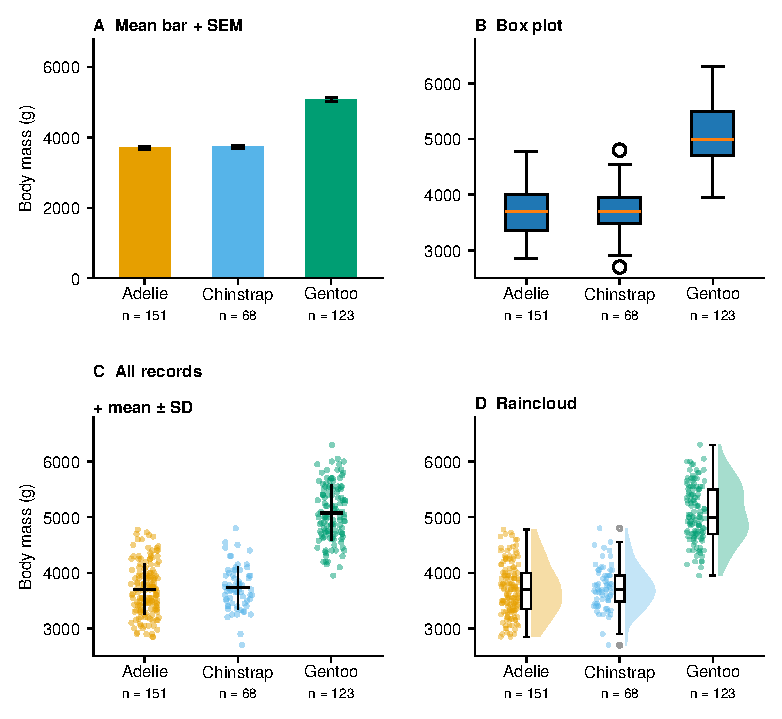
\includegraphics[width=\linewidth]{figures/ch05/ch05-01-group-forms-en.pdf}
\caption{Four views of the same data. Body mass of three penguin species (\texttt{palmerpenguins}; $n = 342$ records after removing 2 records with missing body mass). (A) Mean bars $\pm 1\ \text{SEM}$; (B) box plots with whiskers at $1.5 \times \text{IQR}$; (C) all records with group mean $\pm 1\ \text{SD}$; (D) raincloud plot combining half-violin kernel density, box plot, and jittered raw points. Panel A reduces 342 records to six summary numbers, hiding both the two-fold difference in group sizes and the shape of each distribution.}\label{fig:ch05-01}
\end{figure}

Comparing the four panels of Figure~\ref{fig:ch05-01} shows what each chart reveals or conceals:

\begin{itemize}
\item \textbf{Panel A (Mean bar + SEM): compressing 342 records into 6 numbers.} Panel A starts its vertical axis honestly at $0\ \text{g}$, yet it conveys only three group means ($3700.7\ \text{g}$, $3733.1\ \text{g}$, and $5076.0\ \text{g}$) and three SEMs ($37.3\ \text{g}$, $46.6\ \text{g}$, and $45.5\ \text{g}$). On a six-kilogram scale, the SEM whiskers shrink into tiny black caps. Without the explicit \texttt{n =} labels below the horizontal axis, three equal-width bars would hide the fact that Chinstrap ($n = 68$) has fewer than half as many records as Adelie ($n = 151$). Moreover, no adult penguin weighs between $0\ \text{g}$ and $2700\ \text{g}$, yet solid bars fill that empty zone while compressing the actual data range ($2700\text{--}6300\ \text{g}$) into the upper half of the frame. As Weissgerber et al.\ (2015) showed, identical bar graphs can conceal normal, skewed, bimodal, or outlier-driven distributions; for small-to-moderate sample sizes, authors should plot the individual points.

\item \textbf{Panel B (Box plot): exposing quartiles and extreme points while still hiding $n$ and subpopulations.} Because a box plot encodes values by vertical position rather than bar area from zero, Panel B focuses its vertical axis on $2500\text{--}6800\ \text{g}$. Orange lines mark the medians ($3700\ \text{g}$, $3700\ \text{g}$, and $5000\ \text{g}$), box edges mark the first and third quartiles (interquartile range, IQR), and whiskers extend to $1.5 \times \text{IQR}$. A feature hidden in Panel A now appears: Chinstrap has two open-circle extreme points beyond the whiskers ($2700\ \text{g}$ and $4800\ \text{g}$). However, uniform box widths still hide sample-size differences, and pooling females and males within a species merges any bimodal split into a single box.

\item \textbf{Panel C (All records + mean $\pm$ SD): returning every observation to the reader.} Panel C plots all 342 records as semi-transparent horizontally jittered points alongside a black horizontal tick (mean) and vertical bar ($\pm 1\ \text{SD}$). Three facts are immediately visible: the sky-blue Chinstrap cloud in the middle is sparser than the flanking clouds; individual weights within each species span nearly two kilograms (Adelie $2850\text{--}4775\ \text{g}$, Chinstrap $2700\text{--}4800\ \text{g}$, Gentoo $3950\text{--}6300\ \text{g}$), captured by the $\pm 1\ \text{SD}$ bars; and extreme observations sit naturally at the top and bottom of each cloud without needing arbitrary whisker cut-offs.

\item \textbf{Panel D (Raincloud plot): combining distribution contour, box plot, and raw points.} Following Allen et al.\ (2019), Panel D places horizontally jittered points on the left of each group (``rain''), a narrow white box plot in the centre, and a half-violin kernel density curve truncated at the group's minimum and maximum on the right (``cloud''). The density contour reveals internal clustering: the bluish-green Gentoo density curve on the right exhibits a broad, two-shouldered profile around $4700\ \text{g}$ and $5500\ \text{g}$, hinting at the underlying female and male subpopulations.
\end{itemize}

This leads to a clear selection rule: \textbf{for small-to-moderate group sizes (from a few observations up to a couple of hundred per group), show all raw points alongside a summary statistic (Panel C or D); when group sizes are so large that points fuse into an ink blot, use box, violin, or raincloud plots and print each group's $n$ along the axis.} When instructing \scidraw{} Scientific Visualization (\sdtool{sci-vis}) to plot raw points, specify that \textbf{random jitter must only perturb horizontal x-positions and never alter vertical values}:

\begin{Prompt}
Change the chart to a grouped strip plot: put species (Adelie, Chinstrap, Gentoo)
on the x-axis and Body mass (g) on the y-axis with range 2500 to 6800.
Plot all 342 individual records as semi-transparent points. Jitter points
horizontally only (within 15% of the group spacing) to reduce overlap; do not
alter any vertical y-values. Overlay each group's mean (horizontal tick) and
+/- 1 SD (vertical line), and print n = ... beneath each species name.
\end{Prompt}

\section{What an Error Bar Actually Means}

Compare Panels A and C of Figure~\ref{fig:ch05-01}: both summarize the same 151 Adelie records, so why is the error bar in Panel A a tiny cap of $37.3\ \text{g}$ whereas the vertical bar in Panel C spans $458.6\ \text{g}$ on each side of the mean? Because Panel A plots the standard error of the mean (SEM) and Panel C plots the sample standard deviation (SD). Confusing error-bar metrics—or omitting their definition—is a pervasive flaw in experimental papers (Cumming et al., 2007; Krzywinski and Altman, 2013).

The three common error-bar statistics answer three distinct questions (Table~\ref{tab:ch05-err}):

\begin{table}[htbp]\centering\footnotesize
\setlength{\tabcolsep}{2.5pt}
\renewcommand{\arraystretch}{1.15}
\caption{Meaning, scaling behaviour, and actual half-widths of the three common error-bar statistics on the penguin body-mass data ($n = 342$: Adelie 151, Chinstrap 68, Gentoo 123).}\label{tab:ch05-err}
\begin{tabularx}{\linewidth}{@{}>{\raggedright\arraybackslash}p{20mm}>{\raggedright\arraybackslash}p{22mm}Yccc@{}}
\toprule
\textbf{Error bar} & \textbf{Formula} & \textbf{Question answered and behaviour as $n$ grows} & \textbf{Adelie} & \textbf{Chinstrap} & \textbf{Gentoo} \\
\midrule
Sample SD & $s = \sqrt{\frac{\sum (x_i - \bar{x})^2}{n-1}}$ & \textbf{Biological spread:} How much do individual records vary around the mean? Stabilizes as $n$ grows; does not shrink with larger samples. & $458.6\ \text{g}$ & $384.3\ \text{g}$ & $504.1\ \text{g}$ \\
Standard error (SEM) & $\text{SEM} = s / \sqrt{n}$ & \textbf{Estimation precision:} How precisely does the sample mean estimate the population mean? Shrinks at rate $1/\sqrt{n}$; does not describe individual spread. & $37.3\ \text{g}$ & $46.6\ \text{g}$ & $45.5\ \text{g}$ \\
95\% CI half-width & $t_{0.975,\,n-1} \times \text{SEM}$ & \textbf{Interval estimation:} Half-width of the 95\% confidence interval for the population mean (roughly $2 \times \text{SEM}$ for moderate-to-large $n$). & $73.7\ \text{g}$ & $93.0\ \text{g}$ & $90.0\ \text{g}$ \\
\bottomrule
\end{tabularx}
\end{table}

Three rules follow from Table~\ref{tab:ch05-err}:

First, \textbf{on the same data, SD and SEM can differ by more than ten-fold.} For the 151 Adelie records, $\text{SD} = 458.6\ \text{g}$; dividing by $\sqrt{151} \approx 12.29$ gives $\text{SEM} = 37.3\ \text{g}$, and the 95\% CI half-width is $73.7\ \text{g}$. To show biological variability among individuals, plot SD (or IQR); to show uncertainty around an estimated group mean, plot the 95\% CI. Never choose SEM merely to make error bars look small.

Second, \textbf{every figure with error bars must state both the error-bar type and each group's $n$ in the legend or caption.} Only when both are given can readers interpret the bars or convert between metrics.

Third, \textbf{do not judge statistical significance by whether error bars overlap} (Cumming et al., 2007; Krzywinski and Altman, 2013). When bars show $\pm 1\ \text{SD}$, heavy overlap is still compatible with highly significant mean differences. Conversely, when independent $\pm 1\ \text{SEM}$ bars just touch without overlapping, the two-sided $p$-value is still above $0.05$ (for two independent groups of similar size, $\pm 1\ \text{SEM}$ bars need a gap of roughly $0.5\text{--}1\ \text{SEM}$, or 95\% CI bars must overlap by no more than about one-fourth of one arm, to correspond roughly to $p \le 0.05$).

Because many AI plotting tools default to drawing unlabelled SEM bars, always specify the exact metric in \sdtool{sci-vis}:

\begin{Prompt}
Use sample standard deviation (+/- 1 SD, ddof = 1) for all error bars; do not
use standard error of the mean (SEM). State "Tick: mean; line: +/- 1 SD" in
the legend, print the sample size n below each group on the x-axis, and do not
add significance asterisks or p-values.
\end{Prompt}

\section{Paired and Repeated Measures}

When two columns of numbers come from the same experimental units measured before and after a treatment—or the same sites across two periods—the rows carry a one-to-one \textbf{paired structure}. Returning to the simulated teaching dataset from Chapters 1 and 2 (\texttt{paired-example.csv}, CC BY 4.0), 8 fictional objects (\texttt{SIM01}--\texttt{SIM08}) have a pre-test mean of $13.125\ \text{a.u.}$, a post-test mean of $16.5\ \text{a.u.}$, individual differences ($\text{after} - \text{before}$) of $+4, +3, +4, -1, +4, +5, +4, +4$, and a mean difference of $3.375\ \text{a.u.}$. Figure~\ref{fig:ch05-03} compares three ways of plotting these pairs.

\begin{figure}[htbp]\centering
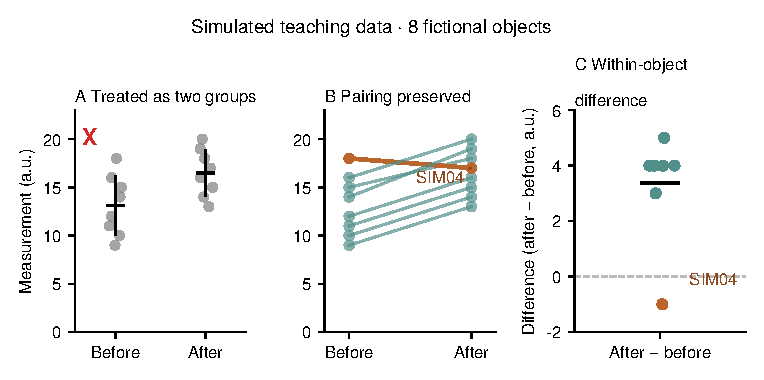
\includegraphics[width=\linewidth]{figures/ch05/ch05-03-paired-views-en.pdf}
\caption{Three ways to plot paired data (simulated teaching data). Eight fictional objects measured twice. (A) Treating the columns as independent groups discards the pairing and suggests 16 objects; (B) connecting each object's two values keeps the decrease of \texttt{SIM04} visible; (C) plotting within-object differences answers ``how much did each change'': seven positive, one negative (\texttt{SIM04} $= -1$), mean difference $3.375\ \text{a.u.}$. No significance test was performed.}\label{fig:ch05-03}
\end{figure}

Inspecting the three panels of Figure~\ref{fig:ch05-03} shows how layout choices either destroy or preserve the pairing:

\begin{itemize}
\item \textbf{Panel A (Treated as two groups, marked with a red \texttt{X}): discarding the pairing.} Panel A plots \texttt{Before} and \texttt{After} as two unlinked clouds of grey dots with mean $\pm 1\ \text{SD}$. First, 16 unlinked dots mislead readers into assuming 16 independent objects were measured. Second, wide baseline variation across objects ($9$ to $18$ before treatment) swamps the within-object change, so the two vertical clouds overlap heavily and hide whether individuals went up or down.

\item \textbf{Panel B (Pairing preserved—paired dot--line plot): exposing individual trajectories.} Panel B connects each object's \texttt{Before} and \texttt{After} values. Seven teal lines climb in parallel ($+3$ to $+5\ \text{a.u.}$), whereas a single object in warm brown—\texttt{SIM04}—starts at the highest baseline ($18$) and drops to $17$ ($-1$). Use Panel B when both initial baseline levels (such as a potential ceiling effect in \texttt{SIM04}) and individual directions of change matter.

\item \textbf{Panel C (Within-object difference plot): directly answering ``how much did each unit change?''} Panel C plots the eight differences ($\text{After} - \text{before}$) on the vertical axis, marks the mean difference ($3.375\ \text{a.u.}$) with a black horizontal tick, and draws a dashed grey reference line at $y = 0$. Seven teal dots sit above zero between $+3$ and $+5$ (the five ties at $+4$ are jittered horizontally), while \texttt{SIM04} sits below zero at $-1$. One rule is mandatory: \textbf{the vertical axis of a difference plot ($-2$ to $6$ here) must include $0$ and display a zero reference line}, because zero separates gains from losses.
\end{itemize}

When plotting paired data with AI tools, guard against two risks: first, the tool ignoring \texttt{sample\_id} and defaulting to Panel A; second, vague prompts like ``clean the data and highlight the main trend'' causing automated scripts to drop the lone decreasing unit \texttt{SIM04} as an ``outlier.'' Always specify: ``Connect observations by \texttt{sample\_id}; retain all 8 objects and never drop counter-trend or extreme observations.''

\section{Time Series and the Dual-Axis Trap}

Time-series plots rest on two rules: \textbf{the horizontal axis must map time continuously in true proportion, and interpolations or methodological changes recorded in the metadata must be marked on the plot.}

We illustrate these rules with the classic atmospheric $\text{CO}_2$ dry-air mole fraction monthly mean record from the Mauna Loa Observatory in Hawaii (Keeling, 1960; maintained by Dr.\ Xin Lan at NOAA GML and Dr.\ Ralph Keeling at Scripps Institution of Oceanography; public domain, WMO X2019 scale). Our locked snapshot (file creation date October 9, 2026) spans 823 monthly rows from March 1958 ($315.71\ \text{ppm}$) to September 2026 ($426.07\ \text{ppm}$), with a minimum monthly mean of $312.42\ \text{ppm}$ and a peak of $432.34\ \text{ppm}$ in May 2026. Figure~\ref{fig:ch05-04} shows the standard presentation of this series.

\begin{figure}[htbp]\centering
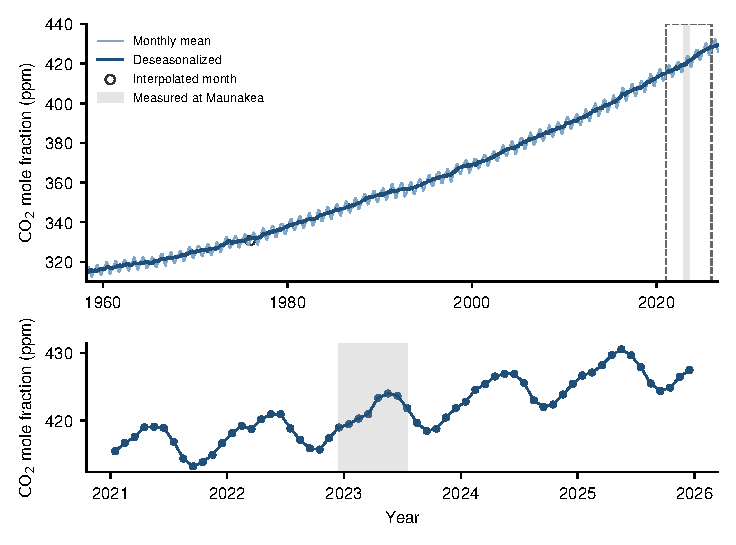
\includegraphics[width=\linewidth]{figures/ch05/ch05-04-co2-series-en.pdf}
\caption{Monthly mean atmospheric $\text{CO}_2$ at Mauna Loa, March 1958 to September 2026 snapshot. Top (full record): thin light-blue line, monthly means (\texttt{average}); thick dark-blue line, NOAA's deseasonalized trend (\texttt{deseasonalized}); open circle, the interpolated month flagged in the data notes (December 1975); grey vertical band, the period after the late-2022 eruption when measurements were made at Maunakea (December 2022--July 2023); dashed box on the right outlines the zoom window. Bottom: the last five complete calendar years (2021--2025), showing the seasonal cycle. Data: NOAA GML (X.\ Lan) and Scripps Institution of Oceanography (R.\ Keeling), snapshot dated October 9, 2026; data before May 1974 are from Scripps.}\label{fig:ch05-04}
\end{figure}

Inspecting Figure~\ref{fig:ch05-04} highlights four time-series standards:

\begin{enumerate}
\item \textbf{Continuous numerical time axis:} The horizontal axis plots \texttt{decimal date} so every month and year is spaced proportionally rather than treated as categorical text labels.
\item \textbf{Raw observations layered with official trend:} The upper panel plots both the thin light-blue monthly mean curve (\texttt{average}) and the thick dark-blue official deseasonalized curve (\texttt{deseasonalized}), without substituting an undocumented smoother.
\item \textbf{Zoomed window for high-frequency cycles:} Over nearly 70 years, seasonal oscillations compress into fine sawteeth. A dashed box on the right of the upper panel marks the last five complete years (2021--2025), expanded in the lower panel (at a $2:1$ height ratio) with monthly dots showing the Northern Hemisphere growing-season cycle (peaking around May, troughing in September--October).
\item \textbf{Marking metadata notes from \texttt{\#} header comments:} Skipping \texttt{\#} comment lines when reading a CSV hides critical provenance. The Mauna Loa header notes two special cases: first, data prior to May 1974 come from Scripps, and since NOAA began independent measurements in May 1974, December 1975 is the only month with zero valid observation days (\texttt{ndays = -1}) due to instrument failure, making its value an interpolation—marked with an open circle (\texttt{Interpolated month}); second, after the late-November 2022 eruption of Mauna Loa cut power and road access, measurements from December 2022 through July 2023 were temporarily taken at the Maunakea summit roughly 21 miles away—shaded with a light-grey vertical band (\texttt{Measured at Maunakea}) in both panels. Only an author who reads the file header can instruct the tool to flag these events.
\end{enumerate}

When comparing two time series with different units or magnitudes, the most common trap is the \textbf{dual-axis chart (twin y-axes)}. Taking the 67 complete calendar years in our snapshot (1959--2025), we compute each year's 12-month arithmetic mean concentration and then the difference between consecutive annual means for 1960--2025 (66 values in $\text{ppm yr}^{-1}$: minimum $0.42$, maximum $3.52\ \text{ppm yr}^{-1}$ in 2024; $0.93\ \text{ppm yr}^{-1}$ in 1960 and $2.74\ \text{ppm yr}^{-1}$ in 2025; note that this consecutive-annual-mean difference differs from NOAA's official December-to-December growth-rate estimator, which the caption must state). Figure~\ref{fig:ch05-06} contrasts a dual-axis plot with stacked panels.

\begin{figure}[htbp]\centering
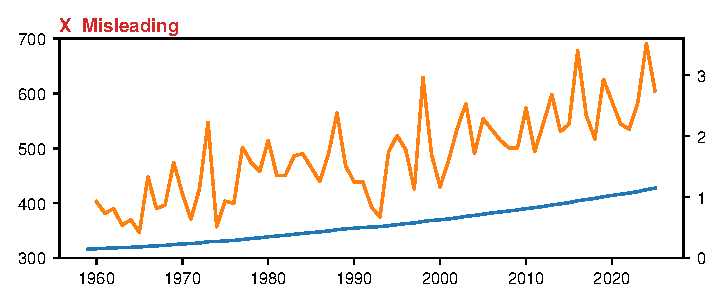
\includegraphics[width=\linewidth]{figures/ch05/ch05-06-dual-axis-bad-en.pdf}\\[4pt]
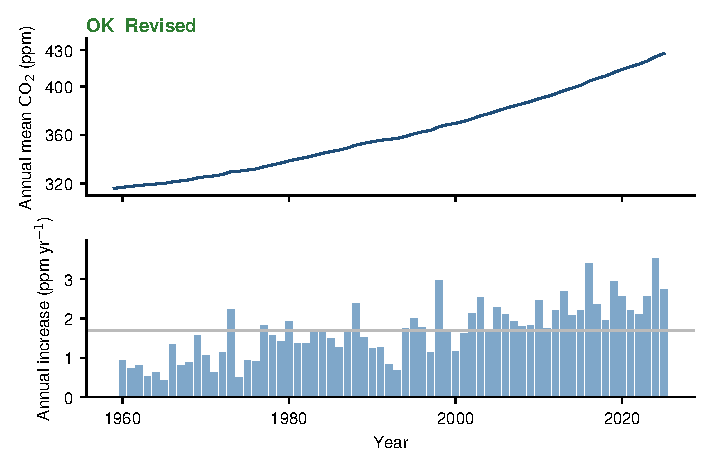
\includegraphics[width=\linewidth]{figures/ch05/ch05-06-dual-axis-good-en.pdf}
\caption{Dual axes versus stacked panels (top: deliberately misleading teaching example). Top: annual mean $\text{CO}_2$ and its annual increase share one plot with two y-axes whose ranges were chosen arbitrarily, so the visual alignment of the curves means nothing. Bottom: each quantity has its own panel on a shared time axis, and the annual increase is plotted from zero. Annual means are averages of NOAA monthly values for complete years (1959--2025); the annual increase is the difference between consecutive annual means, which differs from NOAA's published growth-rate method.}\label{fig:ch05-06}
\end{figure}

In the upper plot of Figure~\ref{fig:ch05-06} (\texttt{X Misleading}), the left axis runs from $300$ to $700\ \text{ppm}$, squashing the rising blue concentration curve against the bottom, while the right axis runs from $0$ to $3.6$ so the orange annual-increase curve fills the frame, with both axes lacking titles and units. Because \textbf{the origin and scale of two vertical axes can be chosen arbitrarily}, altering either axis range can make the two lines cross or run parallel at any year, manufacturing false visual relationships. The lower plot (\texttt{OK Revised}) gives each quantity its own panel above a shared 1959--2025 time axis: the upper panel shows annual mean $\text{CO}_2$ ($310\text{--}440\ \text{ppm}$), and the lower panel shows annual increase as a bar chart starting at $0$ ($0\text{--}4.0\ \text{ppm yr}^{-1}$) with a light-grey reference line at the 1960--2025 mean ($1.69\ \text{ppm yr}^{-1}$).

\section{Scatter Plots and Correlation: When Grouping Flips the Answer}

When examining two continuous variables, omitting categorical grouping variables often leads AI tools to fit a single pooled regression line across all rows—a default that can reverse the scientific conclusion. Figure~\ref{fig:ch05-08} uses penguin bill length (\texttt{bill\_length\_mm}) and bill depth (\texttt{bill\_depth\_mm}, $n = 342$ after removing 2 missing rows) to demonstrate \textbf{Simpson's paradox}.

\begin{figure}[htbp]\centering
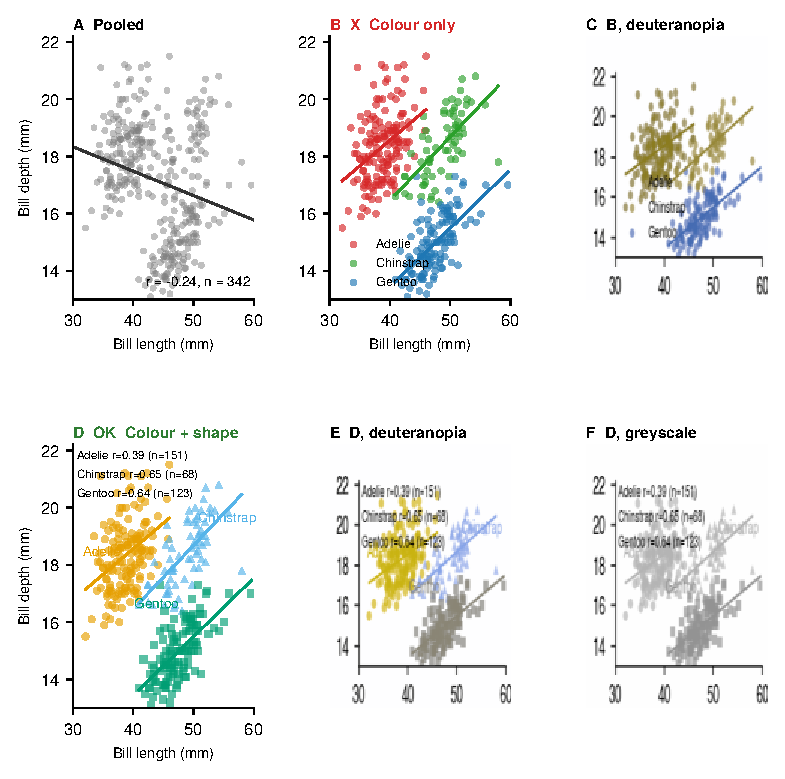
\includegraphics[width=\linewidth]{figures/ch05/ch05-08-scatter-cvd-en.pdf}
\caption{Grouping can reverse a correlation, and group colours must survive checking. Penguin bill length versus bill depth ($n = 342$ records). (A) Pooled, the correlation is negative ($r = -0.24$); (B, D) within each species it is positive ($r = 0.39$, $0.65$, and $0.64$). In (B), species differ only by red, green, and blue circles and become hard to tell apart under simulated deuteranopia (C; Machado et al.\ 2009 model). (D) uses a colour-blind-safe palette, distinct marker shapes, and direct labels, which remain legible under simulation (E) and in greyscale (F). Lines are ordinary least-squares fits, shown descriptively.}\label{fig:ch05-08}
\end{figure}

Compare Panel A and Panel D of Figure~\ref{fig:ch05-08}. In \textbf{Panel A (\texttt{A Pooled})}, all 342 records are mixed into a single cloud of grey dots, and the ordinary least-squares (OLS) line slopes downward ($r = -0.24$, $n = 342$), suggesting that longer bills are shallower.

In \textbf{Panels B and D}, stratifying those same 342 records by species reverses the correlation by 180 degrees: within every species, bill length and depth are positively correlated—Adelie $r = 0.39$ ($n = 151$, upper-left orange circles), Chinstrap $r = 0.65$ ($n = 68$, upper-right sky-blue triangles), and Gentoo $r = 0.64$ ($n = 123$, lower-right bluish-green squares). Panel D shows why: large-bodied Gentoo penguins have relatively long, shallow bills (lower right), whereas Adelie penguins have shorter, deeper bills (upper left); within each species, larger individuals have both longer and deeper bills. The pooled line in Panel A merely connects the centroids of distinct species clusters, mistaking \textbf{between-species divergence} for \textbf{within-species allometry}.

When directing AI tools to make scatter plots, enforce three rules: (1) declare grouping variables up front rather than accepting a pooled fit; (2) report $r$ together with $n$ and the grouping level (as in Panel D) and state the fitting method in the caption; and (3) do not clutter exploratory plots with unadjusted regression $p$-values.

\section{Keeping Charts Honest: Truncated Axes, 3D Bars, Excess Decimals, and Rainbow Colormaps}

Four additional errors frequently distort quantitative charts: \textbf{truncated bar axes, 3D perspective bars, false decimal precision, and rainbow colormaps.}

Figure~\ref{fig:ch05-05} uses the three species mean body masses ($n = 342$) to contrast a chart combining the first three flaws (left) with an honest dot plot of the same values (right).

\begin{figure}[htbp]\centering
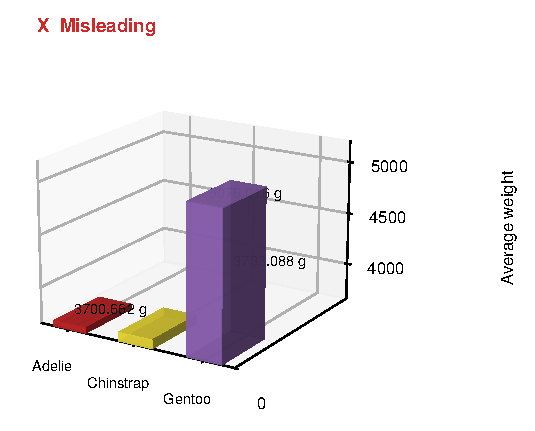
\includegraphics[width=0.49\linewidth]{figures/ch05/ch05-05-axis-bad-en.pdf}\hfill
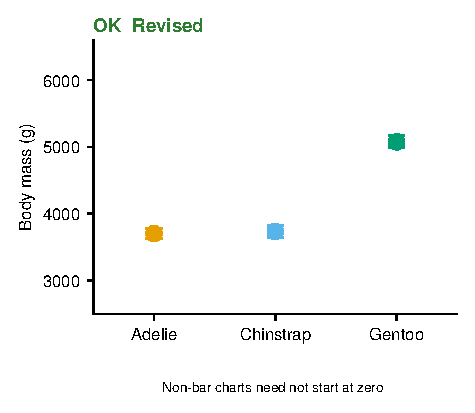
\includegraphics[width=0.49\linewidth]{figures/ch05/ch05-05-axis-good-en.pdf}
\caption{A misleading and an honest view of the same means (deliberately bad example on the left). Left: 3D bars, an axis truncated at $3650\ \text{g}$, rainbow colours, three decimal places, and no unit make a $<1\%$ difference between Adelie and Chinstrap look dramatic. Right: means with 95\% confidence intervals on a labelled axis with integer ticks. Data as in Figure~\ref{fig:ch05-01} ($n = 342$).}\label{fig:ch05-05}
\end{figure}

Inspecting the left panel of Figure~\ref{fig:ch05-05} (\texttt{X Misleading}) reveals three concrete defects:

\begin{enumerate}
\item \textbf{Truncating a bar chart's axis magnifies tiny differences:} Bar charts encode value by bar height and area from a zero baseline, so their axis must start at $0$. Cropping the axis at $3650\ \text{g}$ turns a $32.4\ \text{g}$ difference between Adelie ($3700.7\ \text{g}$) and Chinstrap ($3733.1\ \text{g}$)—less than $0.9\%$—into visible bar heights of $50.7\ \text{g}$ versus $83.1\ \text{g}$ (over 60\% taller), while the purple Gentoo bar ($5076.0\ \text{g}$) towers overhead. The right panel (\texttt{OK Revised}) switches to a \textbf{2D dot plot of means and 95\% CIs}: because dot plots encode value by coordinate position rather than bar area, the vertical axis can span $2500\text{--}6600\ \text{g}$ (as noted at the bottom: \texttt{Non-bar charts need not start at zero}), showing at a glance that Adelie and Chinstrap have nearly identical means with overlapping confidence intervals.
\item \textbf{3D perspective bars distort reading and cause label collisions:} In the 3D plot (\texttt{bar3d}), tilted bar tops make it impossible to tell whether to align the front or back edge with the ticks ($4000, 4500, 5000$) on the right wall; a meaningless \texttt{0} tick appears on the depth axis at bottom right; the vertical title \texttt{Average weight} is pushed to the right margin; and the floating labels \texttt{5076.016 g} and \texttt{3733.088 g} collide with the purple Gentoo bar.
\item \textbf{Excess decimals fabricate precision and units are missing:} Field weights were recorded to the nearest $25\ \text{g}$ or $50\ \text{g}$, yet the left panel prints three decimal places (\texttt{3700.662 g}) and omits units on the axis; the right panel drops redundant in-plot digits and labels the axis \texttt{Body mass (g)} with integer ticks.
\end{enumerate}

The fourth error is the \textbf{rainbow colormap (\texttt{jet})} on continuous matrices. Figure~\ref{fig:ch05-07} arranges Mauna Loa monthly mean $\text{CO}_2$ across 1959--2025 into a $67 \times 12$ matrix ($312.42\text{--}432.34\ \text{ppm}$, unsmoothed) and compares \texttt{jet} with the perceptually uniform colormap \texttt{viridis}.

\begin{figure}[htbp]\centering
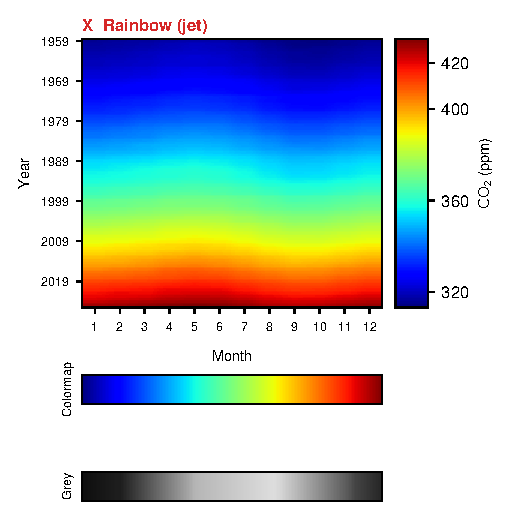
\includegraphics[width=0.49\linewidth]{figures/ch05/ch05-07-colormap-bad-en.pdf}\hfill
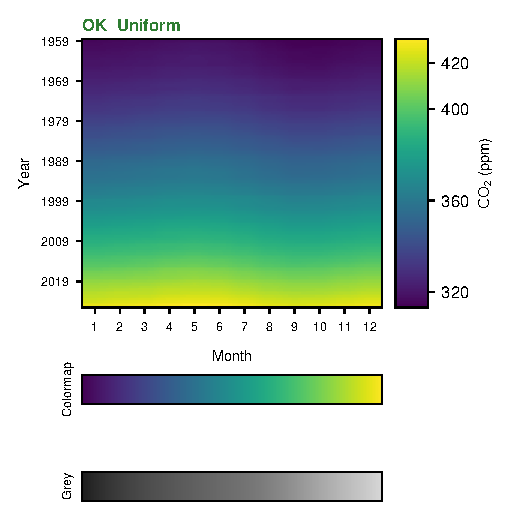
\includegraphics[width=0.49\linewidth]{figures/ch05/ch05-07-colormap-good-en.pdf}
\caption{Rainbow versus perceptually uniform colour maps (left: deliberately bad example). Both heat maps show the same $67 \times 12$ matrix of monthly mean $\text{CO}_2$ at Mauna Loa, 1959--2025. The \texttt{jet} map introduces apparent boundaries at cyan and yellow that are not in the data, and its greyscale strip (\texttt{Grey}) rises then falls in lightness; \texttt{viridis} increases monotonically in lightness and still reads correctly in greyscale.}\label{fig:ch05-07}
\end{figure}

In Figure~\ref{fig:ch05-07}, even though $\text{CO}_2$ rises smoothly over 67 years, the left heatmap (\texttt{X Rainbow (jet)}) creates false sharp bands at bright cyan (around 1989) and bright yellow (around 2009). Worse, its bottom \texttt{Grey} strip shows that luminance in \texttt{jet} rises in the middle and darkens at both ends (deep blue and deep red), scrambling low and high values when printed in black and white (Crameri et al., 2020; Nu\~nez et al., 2018). The right panel (\texttt{OK Uniform}) uses \texttt{viridis} (or \texttt{cividis} for severe colour-vision deficiency), whose \texttt{Grey} strip brightens monotonically from left to right, preserving both the long-term rise and the May-peak / autumn-trough seasonal wave in greyscale.

To fix these flaws in \sdtool{sci-vis}, send a direct prompt:

\begin{Prompt}
1. Replace the 3D bar chart with a 2D plot of group means and 95% confidence
   intervals (if using bars, the y-axis must start at 0). Never use 3D bars.
   Remove the 3-decimal text labels, title the y-axis "Body mass (g)", and use
   integer tick marks.
2. For the heatmap, replace the rainbow (jet) colormap with the perceptually
   uniform colormap viridis (or cividis), and label the colorbar "CO2 (ppm)".
\end{Prompt}

\section{Checking for Colour-Vision Deficiency and Greyscale}

Roughly 8\% of men of Northern European descent have some form of red--green colour-vision deficiency (most commonly deuteranopia or deuteranomaly), and many readers across all populations are affected (Wong, 2011)—and papers are frequently read in greyscale printouts. Categorical groups must never rely on red-versus-green hue alone.

Return to Panels B--F of Figure~\ref{fig:ch05-08}. \textbf{Panel B (\texttt{B X Colour only})} plots all three species as identical circles distinguished only by red, green, and blue. Under physiological deuteranopia simulation (Machado et al., 2009) in \textbf{Panel C (\texttt{C B, deuteranopia})}, the red Adelie and green Chinstrap clouds, regression lines, and legend markers collapse into nearly indistinguishable olive-brown tones. By contrast, \textbf{Panel D (\texttt{D OK Colour + shape})} combines three defences: (1) the Okabe--Ito palette (\texttt{\#E69F00}, \texttt{\#56B4E9}, \texttt{\#009E73}); (2) \textbf{redundant marker shapes} (circles \texttt{o} for Adelie, triangles \texttt{\^{}} for Chinstrap, squares \texttt{s} for Gentoo); and (3) \textbf{direct species labels} beside each cloud (note also that at final print scale one should check label placement—in Panel D the correlation text at upper left sits near the highest Adelie circles and the direct species names sit snug against the clouds, which can be nudged if needed). With this triple encoding, all three groups remain clear under simulated deuteranopia (\textbf{Panel E}) and in greyscale (\textbf{Panel F}).

Before submission, upload exported figures to \scidraw{} Figure Checker (\sdtool{figure-checker}) for automated greyscale and colour-vision simulation checks—remembering that technical checks never replace scientific review (such as catching Simpson's paradox in Panel A).

\section{End-to-End Case Study: Completing a Penguin Body-Mass Figure with SciDraw AI}

We now complete Lin Yue's opening task: using \path{penguins.csv}, build a figure for the ``Study System'' subsection and lab-meeting slides showing adult breeding body mass across the three \emph{Pygoscelis} species (Adelie \emph{P.\ adeliae}, Chinstrap \emph{P.\ antarcticus}, Gentoo \emph{P.\ papua}) stratified by species and sex. First, we fix the scientific boundary: \textbf{this figure is a purely descriptive morphological display; no inferential statistical tests are run, and no asterisks or $p$-values are drawn.}

\textbf{Step 1: Independently compute benchmark values.} Following Table~\ref{tab:ch05-dict}, dropping the 11 rows where \texttt{sex} or \texttt{body\_mass\_g} is \texttt{NA} leaves \textbf{$n = 333$} records. Before using AI, we compute the sample size, mean, and sample SD ($\text{ddof} = 1$) for all six species $\times$ sex subgroups (Table~\ref{tab:ch05-case-expect}; pooled species values are in Table~\ref{tab:ch05-err}). Comparing the two tables shows that within every species, males average $412\text{--}805\ \text{g}$ heavier than females, and within-sex SDs ($269.4\text{--}362.1\ \text{g}$) are much smaller than pooled-sex SDs ($384.3\text{--}504.1\ \text{g}$), confirming that much of the pooled spread comes from sexual dimorphism.

\begin{table}[htbp]\centering\footnotesize
\setlength{\tabcolsep}{4pt}
\renewcommand{\arraystretch}{1.15}
\caption{Verification benchmark table of penguin body mass by species $\times$ sex (excluding 11 rows with missing sex or body mass; $n = 333$).}\label{tab:ch05-case-expect}
\begin{tabularx}{\linewidth}{@{}llccY@{}}
\toprule
\textbf{Species (common and scientific name)} & \textbf{Sex} & \textbf{Records $n$} & \textbf{Mean (g)} & \textbf{Sample SD (g)} \\
\midrule
Adelie (\emph{P.\ adeliae}) & \texttt{female} & 73 & 3368.8 & 269.4 \\
Adelie (\emph{P.\ adeliae}) & \texttt{male}   & 73 & 4043.5 & 346.8 \\
Chinstrap (\emph{P.\ antarcticus}) & \texttt{female} & 34 & 3527.2 & 285.3 \\
Chinstrap (\emph{P.\ antarcticus}) & \texttt{male}   & 34 & 3939.0 & 362.1 \\
Gentoo (\emph{P.\ papua}) & \texttt{female} & 58 & 4679.7 & 281.6 \\
Gentoo (\emph{P.\ papua}) & \texttt{male}   & 61 & 5484.8 & 313.2 \\
\bottomrule
\end{tabularx}
\end{table}

\textbf{Step 2: Draft the figure brief in the Figure Workflow Guide.} In \scidraw{} Figure Workflow Guide (\sdtool{figure-workflow}), select the ``Data Figure'' route, replace the default brief with the specification below, download a copy, and proceed to Scientific Visualization (\sdtool{sci-vis}):

\begin{Prompt}
[Research Question] How does adult body mass distribute across three Pygoscelis
                    penguin species, and how much do females and males differ
                    within each species?
[Purpose & Audience] Descriptive figure for the paper's "Study System" section
                     (single-column width ~85 mm) plus lab-meeting slides;
                     audience is ecology peers.
[Data Source] Public dataset: penguins.csv from palmerpenguins v0.1.0 (CC0),
              Palmer Station LTER, 2007-2009.
[Fields & Units] species (group), sex (subgroup), body_mass_g (Body mass, g).
[Unit of Observation & n] Each row is one measurement record. Exclude the 11 rows
              where sex or body_mass_g is NA, retaining n = 333 records. Print
              each subgroup's n beneath the x-axis.
[Pairing] None. Records are unlinked; do not connect points with lines.
[Visual Encoding] Grouped strip plot: arrange species as Adelie, Chinstrap,
              Gentoo; place female on the left and male on the right within each.
[Summary & Error Bars] Show all raw points (jittered horizontally only; y-values
              unchanged). Overlay group mean +/- 1 SD. No tests, asterisks, or p.
[Forbidden Operations] Do not fabricate, drop, or alter values; do not remove
              "outliers" or impute missing rows.
[Labels & Export] Y-axis "Body mass (g)" with integer ticks; open circles for
              females, filled circles for males; colour-blind-safe species palette;
              legend stating "Tick: mean; line: +/- 1 SD". Export PNG and PDF.
[Acceptance] Subgroup n = 73, 73, 34, 34, 58, 61; means match benchmark table.
\end{Prompt}

\textbf{Step 3: Upload data and audit the first draft.} In Scientific Visualization (\sdtool{sci-vis}), upload \path{penguins.csv} (supports CSV, TSV, TXT, XLSX, XLS, and pasted tables; Excel reads only the first worksheet) and confirm that the interface reports 344 rows $\times$ 8 columns. The platform checks the file hash, byte size, and row count and lets you download the stored raw file to verify that the plot uses your exact table—\textbf{but file integrity does not guarantee appropriate statistical choices.} Paste the brief requirements to generate the first draft, then check it against Table~\ref{tab:ch05-case-expect} for five typical first-draft issues: (1) mean bars + unspecified error bars (often SEM); (2) sexes pooled, or \texttt{sex = NA} plotted as a third sex group \texttt{"NA"}; (3) bar axis truncated above zero; (4) mean labels with 1--3 decimals; and (5) red/green or default colours without open/filled sex markers.

\textbf{Step 4: Issue step-by-step revision prompts and use version rollback.} Address one category of issue per conversational turn. First, send Revision Prompt M1 (chart type and NA filtering):

\begin{Prompt}
Switch to a strip plot where each point represents one measurement record. Order
the x-axis as Adelie, Chinstrap, Gentoo, with females on the left and males on
the right within each species. Jitter points horizontally only (width no more
than 15% of the group spacing) without changing any y-values. Exclude rows where
sex or body_mass_g is NA so no "NA" group appears. Draw no bars; keep all other
settings unchanged.
\end{Prompt}

Second, send Revision Prompt M2 (summary overlay and sample-size labels):

\begin{Prompt}
To the right of each subgroup point cloud, overlay a short horizontal tick for
the group mean and a vertical line for mean +/- 1 SD (sample standard deviation,
ddof = 1). Beneath the x-axis, print each subgroup's sample size (for example,
"n = 73"). In the legend, state "Tick: mean; line: +/- 1 SD". Do not add
significance asterisks, p-values, or test results. Change only these items.
\end{Prompt}

Third, send Revision Prompt M3 (axis settings, integer ticks, and colour-blind-safe palette):

\begin{Prompt}
Set the y-axis title to "Body mass (g)" with range 2500 to 6500, tick interval
500, and integer tick labels (no decimals). Use a colour-blind-safe palette by
species: Adelie orange #E69F00, Chinstrap sky blue #56B4E9, Gentoo bluish green
#009E73; use open circles for females and filled circles for males. Do not alter
the species order or any data values.
\end{Prompt}

Note: conversational editing does not lock unmentioned elements. If M3 inadvertently alters the species order or point positions, do not pile patch prompts onto the broken chart—click ``Restore Previous Version'' (or select the prior state from the ``History'' sidebar) and split M3 into two narrower prompts (first axis settings, then palette and markers). Always re-check unmentioned elements after every turn.

\textbf{Step 5: Final verification, caption, and deliverable folder.} The platform renders charts via a declarative engine or Python backend; the current UI does not provide full script downloads, and declarative PDF/EPS exports may wrap raster content (do not assume every PDF is an editable vector graphic; native Excel chart export is available for supported chart types). We therefore cross-check the reference final figure (Figure~\ref{fig:ch05-02}) against Table~\ref{tab:ch05-case-expect}: x-axis ordered Adelie, Chinstrap, Gentoo; within each species, females on the left (open circles) and males on the right (filled circles), jittered horizontally only; black horizontal ticks and vertical lines to the right of each cloud matching the benchmark means $\pm 1\ \text{SD}$; and two rows of sample sizes beneath each species name (upper row for left/female groups: $n = 73, 34, 58$; lower row for right/male groups: $n = 73, 34, 61$, totaling $333$ with no \texttt{NA} group).

\begin{figure}[htbp]\centering
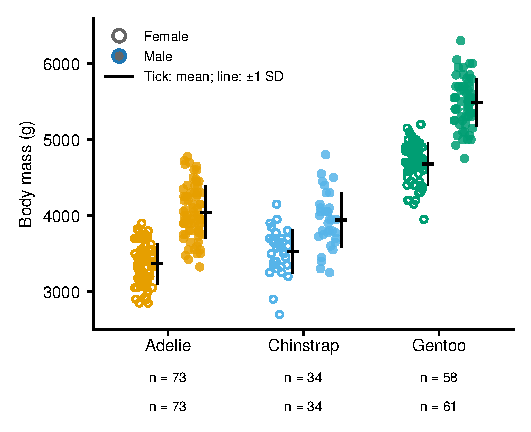
\includegraphics[width=0.68\linewidth]{figures/ch05/ch05-02-case-final-en.pdf}
\caption{Body mass of adult \emph{Pygoscelis} penguins by species and sex. Each point is one measurement record (Palmer Station LTER, 2007--2009; \texttt{palmerpenguins} v0.1.0, CC0). After excluding 11 records with missing sex or body mass, $n = 333$; group sizes are shown beneath the axis (upper row: females; lower row: males). Horizontal ticks show means and vertical lines $\pm 1\ \text{SD}$ (sample standard deviation). Points are jittered horizontally only; values are unchanged. Descriptive display; no statistical tests were performed.}\label{fig:ch05-02}
\end{figure}

If \sdtool{figure-legend} is used to draft a caption, the author must supply the data source and licence, $n = 333$ after excluding 11 missing records, the mean $\pm 1\ \text{SD}$ definition, horizontal-only jitter, and the note that no statistical tests were performed. Archive all deliverables in a structured folder (the example figures in this chapter were generated by deterministic scripts; prompts and verification records are available in the book repository):

\begin{Prompt}
penguin-mass-figure/
  source/   penguins.csv, penguins-README.md, SHA-256.txt
  brief/    figure-brief.txt, data-dictionary.md, benchmark-table.csv
  drafts/   scivis-v1.png ... scivis-v4.png, revision-prompts.md (inputs + audit notes)
  check/    independent verification output check.json, figure-checker report
  final/    figure-5-2.png, figure-5-2.pdf, caption-zh.txt, caption-en.txt, ai-usage.txt
\end{Prompt}

\section{What AI Can and Cannot Do at This Stage}

Table~\ref{tab:ch05-02} summarizes what AI visualization tools can and cannot do, and what the author must verify.

\begin{table}[htbp]\centering\footnotesize
\setlength{\tabcolsep}{3pt}
\renewcommand{\arraystretch}{1.12}
\caption{What AI can do, what it cannot do, and what the author must verify across the data-visualization workflow.}\label{tab:ch05-02}
\begin{tabularx}{\linewidth}{@{}>{\raggedright\arraybackslash}p{19mm}YYY@{}}
\toprule
\textbf{Stage} & \textbf{What AI (\scidraw{} \sdtool{sci-vis}) can do} & \textbf{Cannot do / do not delegate} & \textbf{What the author must verify} \\
\midrule
Reading data & Parse CSV/TSV/TXT/XLSX/XLS and pasted tables; verify hash, byte size, and row count & Know which rows belong to the same individual or which column is a pairing key; infer why values are missing; Excel reads only the first sheet & Row count, column names, and \texttt{NA} counts match the raw file; unit of observation is written in the brief \\
Choosing a chart & Draw strip, box, dot--line, line, or heatmap charts on command; suggest candidates & Understand study design (independent, paired, repeated) unless told; UI does not show rationale for chart suggestions & Chart type matches study design; raw points are shown whenever sample size permits \\
Summaries \& error bars & Compute and plot means, SD, SEM, and CIs & Decide which error bar is scientifically appropriate; guarantee statistical test validity & Error-bar type is stated in legend and caption; $n$ matches the plot; no unrequested asterisks or $p$-values \\
Multi-turn editing & Change chart type, labels, colours, and axes in chat; branch from history; restore previous version & Guarantee that unmentioned elements stay untouched; lock individual canvas objects & After every turn, re-check unmentioned elements (order, values, axis range) \\
Colour \& legibility & Apply specified palettes and column-width styles; run greyscale and CVD simulations in \sdtool{figure-checker} & Judge whether colours carry scientific meaning; technical checks are not scientific review & Groups remain distinct under CVD simulation and greyscale; colormap fits data type \\
Exporting & Download PNG, TIFF, PDF, EPS, and stored raw data; export native Excel charts for supported types & Provide full plotting code downloads in current UI; PDF/EPS is not always an editable vector file & Inspect exported dimensions, fonts, and vector vs.\ raster status; match raw-data hash to local file \\
Figure captions & \sdtool{figure-legend} drafts a layout description from image pixels & Know $n$, exclusion rules, error-bar meaning, or data source (it only sees pixels) & Supply data source, $n$, missing-data handling, error-bar type, and whether tests were run \\
\bottomrule
\end{tabularx}
\end{table}

\section{Chapter Checklist}

\begin{itemize}
\item What each row represents is written in the figure brief; ``number of records'' and ``number of individuals'' are not conflated.
\item Missing-value handling is stated explicitly; no \texttt{"NA"} group appears on the plot; excluded row counts are reported in the caption.
\item Chart type matches the study design: paired data preserve pairing links, time axes are continuous numbers, and grouping variables are visible.
\item When group sizes are small to moderate ($n \le$ a few dozen), all raw points are shown and jitter is strictly horizontal.
\item Error-bar type (SD / SEM / 95\% CI) is written in the legend or caption, and $n$ matches the plot.
\item Bar-chart vertical axes start at $0$; non-bar axis ranges are justified and do not exaggerate differences.
\item There are no dual y-axes, 3D bars, or false decimal places.
\item Continuous data use a perceptually uniform colormap; group colours pass colour-vision and greyscale checks with shape or label redundancy.
\item Every number on the plot has been cross-checked against an independent calculation (script or spreadsheet).
\item Saved in the archive: raw data and its hash, figure brief, every prompt and screenshot, final files, caption, and verification log.
\item Simulated data are labelled as ``simulated teaching data'' on the plot or in the caption.
\end{itemize}

\section{Exercises}

\begin{enumerate}
\item \textbf{Reading a table and choosing a chart (pen and paper):} Given \path{flipper_length_mm} and \texttt{island} in Palmer Penguins, write a data dictionary (including \texttt{NA} counts), tabulate the species composition on each island (Torgersen: 52 Adelie; Biscoe: 44 Adelie $+$ 124 Gentoo; Dream: 56 Adelie $+$ 68 Chinstrap), explain why ``comparing flipper length across the three islands'' is confounded with species (Gentoo occurs only on Biscoe, Chinstrap only on Dream), and propose a non-misleading chart (for example, faceting by island and colouring by species).
\item \textbf{Hands-on practice in \scidraw{}:} Upload \texttt{paired-example.csv} to \sdtool{sci-vis}, first enter only ``Make a before-and-after comparison chart,'' and record the first draft; then follow the logic of Figure~\ref{fig:ch05-03} through chat prompts to obtain both a paired dot--line plot and a difference plot (with vertical axis including $0$), using ``Restore Previous Version'' at least once. Submit: each prompt, screenshot, and a verification table checking all 8 differences (\texttt{SIM04} $= -1$).
\item \textbf{Fixing a misleading chart:} Using this chapter's $\text{CO}_2$ snapshot, create a flawed ``rainbow colormap + dual y-axis'' chart, then write three revision prompts that could be sent directly to an AI tool to fix it; explain how you confirm that the underlying values did not change after revision (for example, by cross-checking an annual-mean table).
\end{enumerate}

\section*{References}

\begin{itemize}
\item Allen M, Poggiali D, Whitaker K, Marshall TR, Kievit RA. Raincloud plots: a multi-platform tool for robust data visualization. \emph{Wellcome Open Research}. 2019;4:63. \url{https://doi.org/10.12688/wellcomeopenres.15191.1}
\item ColorBrewer 2.0: color advice for cartography and scientific visualization. \url{https://colorbrewer2.org/}
\item Crameri F, Shephard GE, Heron PJ. The misuse of colour in science communication. \emph{Nature Communications}. 2020;11:5444. \url{https://doi.org/10.1038/s41467-020-19160-7}
\item Cumming G, Fidler F, Vaux DL. Error bars in experimental biology. \emph{Journal of Cell Biology}. 2007;177(1):7--11. \url{https://doi.org/10.1083/jcb.200611141}
\item Gorman KB, Williams TD, Fraser WR. Ecological sexual dimorphism and environmental variability within a community of Antarctic penguins (genus \emph{Pygoscelis}). \emph{PLoS ONE}. 2014;9(3):e90081. \url{https://doi.org/10.1371/journal.pone.0090081}
\item Horst AM, Hill AP, Gorman KB. palmerpenguins: Palmer Archipelago (Antarctica) penguin data (v0.1.0) [R package]. Zenodo; 2020. \url{https://doi.org/10.5281/zenodo.3960218}
\item Keeling CD. The concentration and isotopic abundances of carbon dioxide in the atmosphere. \emph{Tellus}. 1960;12(2):200--203. \url{https://doi.org/10.3402/tellusa.v12i2.9366}
\item Krzywinski M, Altman N. Points of significance: error bars. \emph{Nature Methods}. 2013;10(10):921--922. \url{https://doi.org/10.1038/nmeth.2659}
\item Lan X, Keeling R. Trends in atmospheric carbon dioxide: Mauna Loa monthly mean data. NOAA Global Monitoring Laboratory and Scripps Institution of Oceanography. \url{https://gml.noaa.gov/ccgg/trends/data.html}
\item Machado GM, Oliveira MM, Fernandes LAF. A physiologically-based model for simulation of color vision deficiency. \emph{IEEE Transactions on Visualization and Computer Graphics}. 2009;15(6):1291--1298. \url{https://doi.org/10.1109/TVCG.2009.113}
\item Nu\~nez JR, Anderton CR, Renslow RS. Optimizing colormaps with consideration for color vision deficiency to enable accurate interpretation of scientific data. \emph{PLoS ONE}. 2018;13(7):e0199239. \url{https://doi.org/10.1371/journal.pone.0199239}
\item Okabe M, Ito K. Color Universal Design (CUD): how to make figures and presentations that are friendly to colorblind people. \url{https://jfly.uni-koeln.de/color/}
\item Rougier NP, Droettboom M, Bourne PE. Ten simple rules for better figures. \emph{PLoS Computational Biology}. 2014;10(9):e1003833. \url{https://doi.org/10.1371/journal.pcbi.1003833}
\item Weissgerber TL, Milic NM, Winham SJ, Garovic VD. Beyond bar and line graphs: time for a new data presentation paradigm. \emph{PLOS Biology}. 2015;13(4):e1002128. \url{https://doi.org/10.1371/journal.pbio.1002128}
\item Wong B. Points of view: color blindness. \emph{Nature Methods}. 2011;8(6):441. \url{https://doi.org/10.1038/nmeth.1618}
\end{itemize}

% TODO: Pending live UI and iterative session screenshots from SciDraw AI Scientific Visualization (/sci-vis) (not yet on disk, so omitted from the main text):
% - figures/ch05/ch05-scivis-v1.png (initial draft screenshot in /sci-vis)
% - figures/ch05/ch05-scivis-v2.png ... ch05-scivis-v4.png (multi-turn conversational edits and version-restore screenshots)
